% =============================================================================
% PART B - MODULE 27: CONVERSATION MANAGEMENT (UC-29.01 - UC-29.08)
% In Charge: Pham Kha Vy
% =============================================================================
\subsection{Module 27: Conversation Management}

\subsubsection{M27.01 -- View Conversation List (UC-29.01)}
\begin{itemize}[leftmargin=1.5em,itemsep=2pt]
  \item \textbf{Screen Name \& Route Path:} Messages -- \texttt{/messages}.
  \item \textbf{Who Can Use This:} Client, Freelancer.
  \item \Needspace{6\baselineskip}\textbf{Before You Begin:} User is signed in to an active account.
\end{itemize}
\begin{figure}[H]\centering
  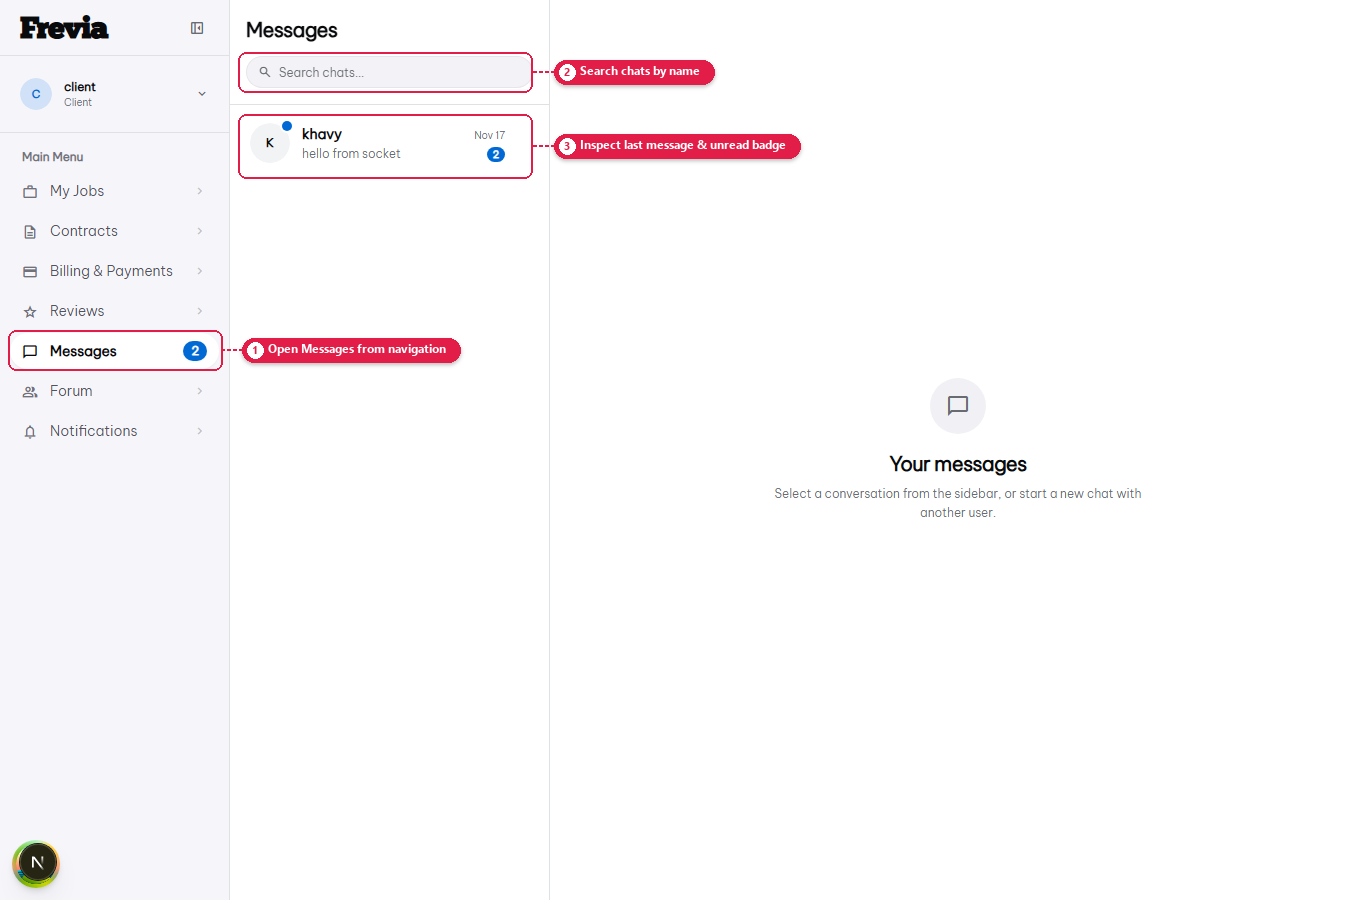
\includegraphics[width=0.90\textwidth]{images/conversation/c27_01_guide.png}
  \caption{Conversation list with last message preview and unread count}
\end{figure}
\Needspace{6\baselineskip}\paragraph{Step-by-Step User Guide:}
\begin{enumerate}[leftmargin=1.8em,itemsep=3pt]
  \item \rbadge{1} \textbf{Open Messages:} Click \textbf{Messages} in the left navigation sidebar.
  \item \rbadge{2} \textbf{Search Conversations:} Type a participant name in the search bar to filter your chat threads.
  \item \rbadge{3} \textbf{Inspect Unread Badges:} Review the latest message preview and blue unread counter badge, then click a thread to open.
\end{enumerate}
\Needspace{6\baselineskip}\paragraph{After You Submit (Result \& Troubleshooting):}
\begin{itemize}[leftmargin=1.5em,itemsep=2pt]
  \item \textbf{What Happens Next:} All active conversations are displayed sorted by pinned status and latest activity.
  \item \textbf{Troubleshooting \& Common Messages:} If no conversations exist yet, an empty inbox prompt is displayed.
\end{itemize}

\subsubsection{M27.02 -- Start Conversation (UC-29.02)}
\begin{itemize}[leftmargin=1.5em,itemsep=2pt]
  \item \textbf{Screen Name \& Route Path:} Messages -- \texttt{/messages}.
  \item \textbf{Who Can Use This:} Client, Freelancer.
  \item \Needspace{6\baselineskip}\textbf{Before You Begin:} User is signed in and selects a target Freelancer or Client.
\end{itemize}
\begin{figure}[H]\centering
  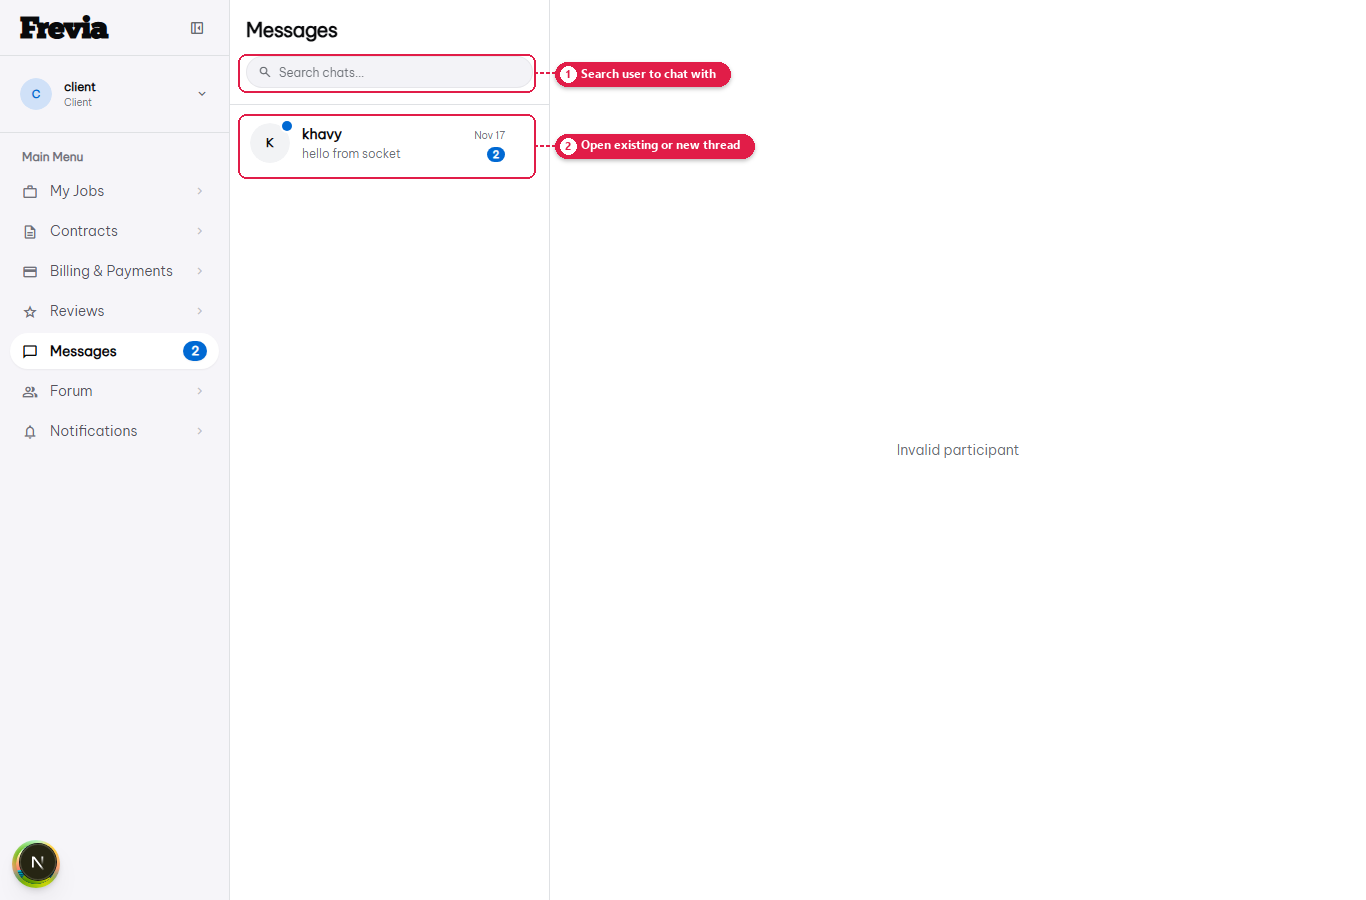
\includegraphics[width=0.90\textwidth]{images/conversation/c27_02_guide.png}
  \caption{Starting or resuming a direct conversation}
\end{figure}
\Needspace{6\baselineskip}\paragraph{Step-by-Step User Guide:}
\begin{enumerate}[leftmargin=1.8em,itemsep=3pt]
  \item \rbadge{1} \textbf{Search or Select Contact:} Use \textit{Search chats...} or click \textbf{Message} from a user profile/proposal to open a conversation.
  \item \rbadge{2} \textbf{Compose Opening Message:} Type an introductory greeting in the bottom message input box.
  \item \rbadge{3} \textbf{Click Send:} Click the blue \textbf{Send} icon to create the 1-on-1 thread and transmit the first message.
\end{enumerate}
\Needspace{6\baselineskip}\paragraph{After You Submit (Result \& Troubleshooting):}
\begin{itemize}[leftmargin=1.5em,itemsep=2pt]
  \item \textbf{What Happens Next:} A unique 1-on-1 conversation thread is created (or the existing thread is opened automatically).
  \item \textbf{Troubleshooting \& Common Messages:} Messaging yourself is disallowed.
\end{itemize}

\subsubsection{M27.03 -- View Conversation Detail (UC-29.03)}
\begin{itemize}[leftmargin=1.5em,itemsep=2pt]
  \item \textbf{Screen Name \& Route Path:} Conversation Thread -- \texttt{/messages}.
  \item \textbf{Who Can Use This:} Client, Freelancer.
  \item \Needspace{6\baselineskip}\textbf{Before You Begin:} User is a participant in the conversation.
\end{itemize}
\begin{figure}[H]\centering
  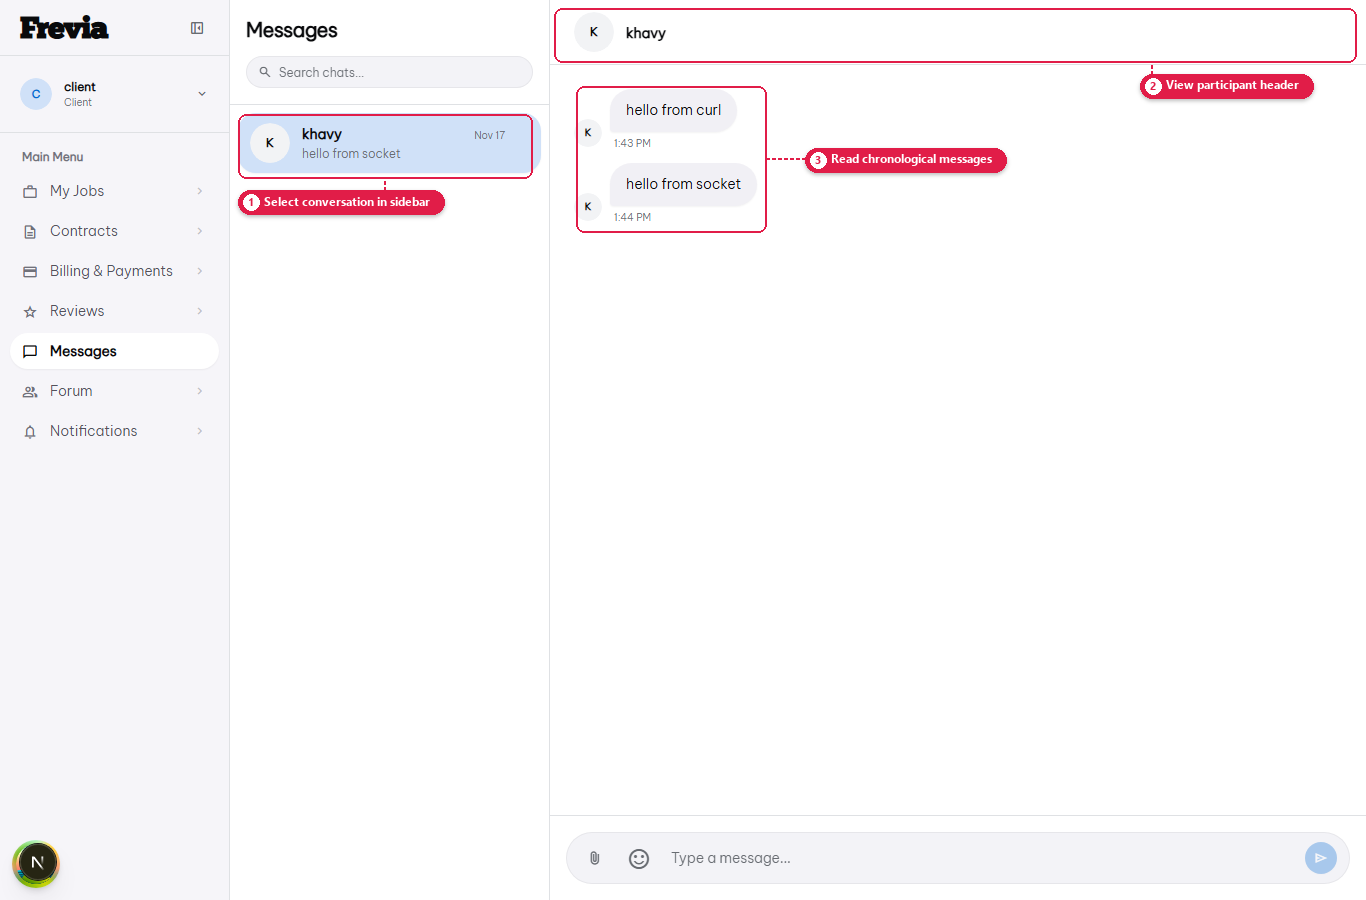
\includegraphics[width=0.90\textwidth]{images/conversation/c27_03_guide.png}
  \caption{Full chronological message thread view}
\end{figure}
\Needspace{6\baselineskip}\paragraph{Step-by-Step User Guide:}
\begin{enumerate}[leftmargin=1.8em,itemsep=3pt]
  \item \rbadge{1} \textbf{Select Thread:} Click a conversation item in the left sidebar.
  \item \rbadge{2} \textbf{View Header:} Confirm the recipient's name and avatar in the top chat header.
  \item \rbadge{3} \textbf{Read Message History:} Scroll through chronological messages, timestamps, and attachment cards.
\end{enumerate}
\Needspace{6\baselineskip}\paragraph{After You Submit (Result \& Troubleshooting):}
\begin{itemize}[leftmargin=1.5em,itemsep=2pt]
  \item \textbf{What Happens Next:} The complete message history loads with sender metadata and read status.
  \item \textbf{Troubleshooting \& Common Messages:} Non-participants cannot access private conversation threads.
\end{itemize}

\subsubsection{M27.04 -- Send Message (UC-29.04)}
\begin{itemize}[leftmargin=1.5em,itemsep=2pt]
  \item \textbf{Screen Name \& Route Path:} Chat Composer -- \texttt{/messages}.
  \item \textbf{Who Can Use This:} Client, Freelancer.
  \item \Needspace{6\baselineskip}\textbf{Before You Begin:} A conversation thread is open.
\end{itemize}
\begin{figure}[H]\centering
  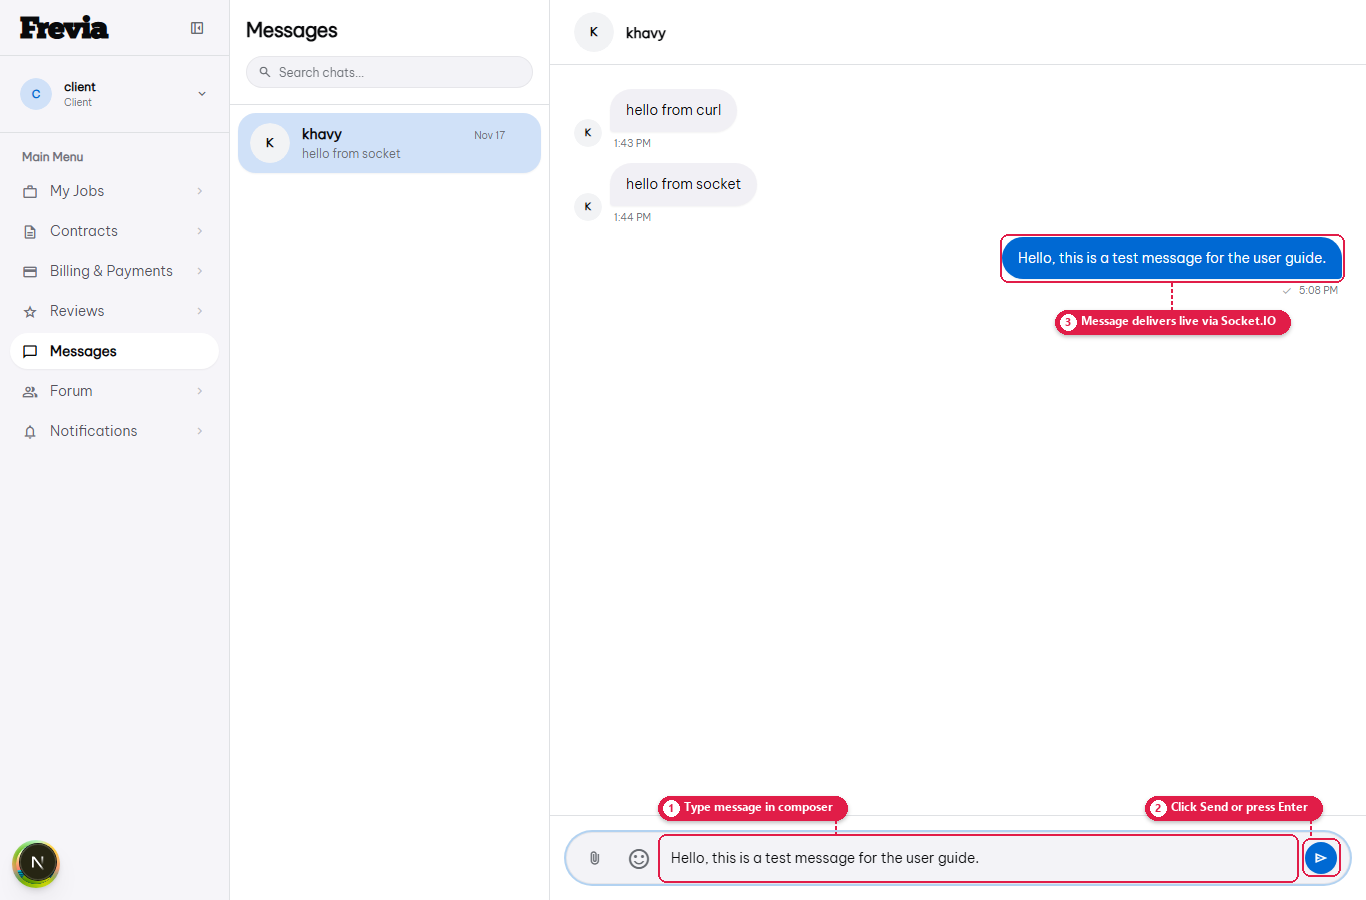
\includegraphics[width=0.90\textwidth]{images/conversation/c27_04_guide.png}
  \caption{Sending a real-time text message via Socket.IO}
\end{figure}
\Needspace{6\baselineskip}\paragraph{Step-by-Step User Guide:}
\begin{enumerate}[leftmargin=1.8em,itemsep=3pt]
  \item \rbadge{1} \textbf{Compose Message:} Click the \textit{Type a message...} input box and enter your text.
  \item \rbadge{2} \textbf{Click Send:} Click the blue \textbf{Send} icon (or press \texttt{Enter}).
  \item \rbadge{3} \textbf{Verify Instant Delivery:} Confirm your blue message bubble renders immediately with delivery timestamp.
\end{enumerate}
\Needspace{6\baselineskip}\paragraph{After You Submit (Result \& Troubleshooting):}
\begin{itemize}[leftmargin=1.5em,itemsep=2pt]
  \item \textbf{What Happens Next:} The message is persisted and broadcast instantaneously over WebSocket.
  \item \textbf{Troubleshooting \& Common Messages:} Empty messages cannot be sent; offline errors display a retry prompt.
\end{itemize}

\subsubsection{M27.05 -- Mark Message as Read (UC-29.05)}
\begin{itemize}[leftmargin=1.5em,itemsep=2pt]
  \item \textbf{Screen Name \& Route Path:} Conversation Thread -- \texttt{/messages}.
  \item \textbf{Who Can Use This:} Client, Freelancer.
  \item \Needspace{6\baselineskip}\textbf{Before You Begin:} Conversation contains unread incoming messages.
\end{itemize}
\begin{figure}[H]\centering
  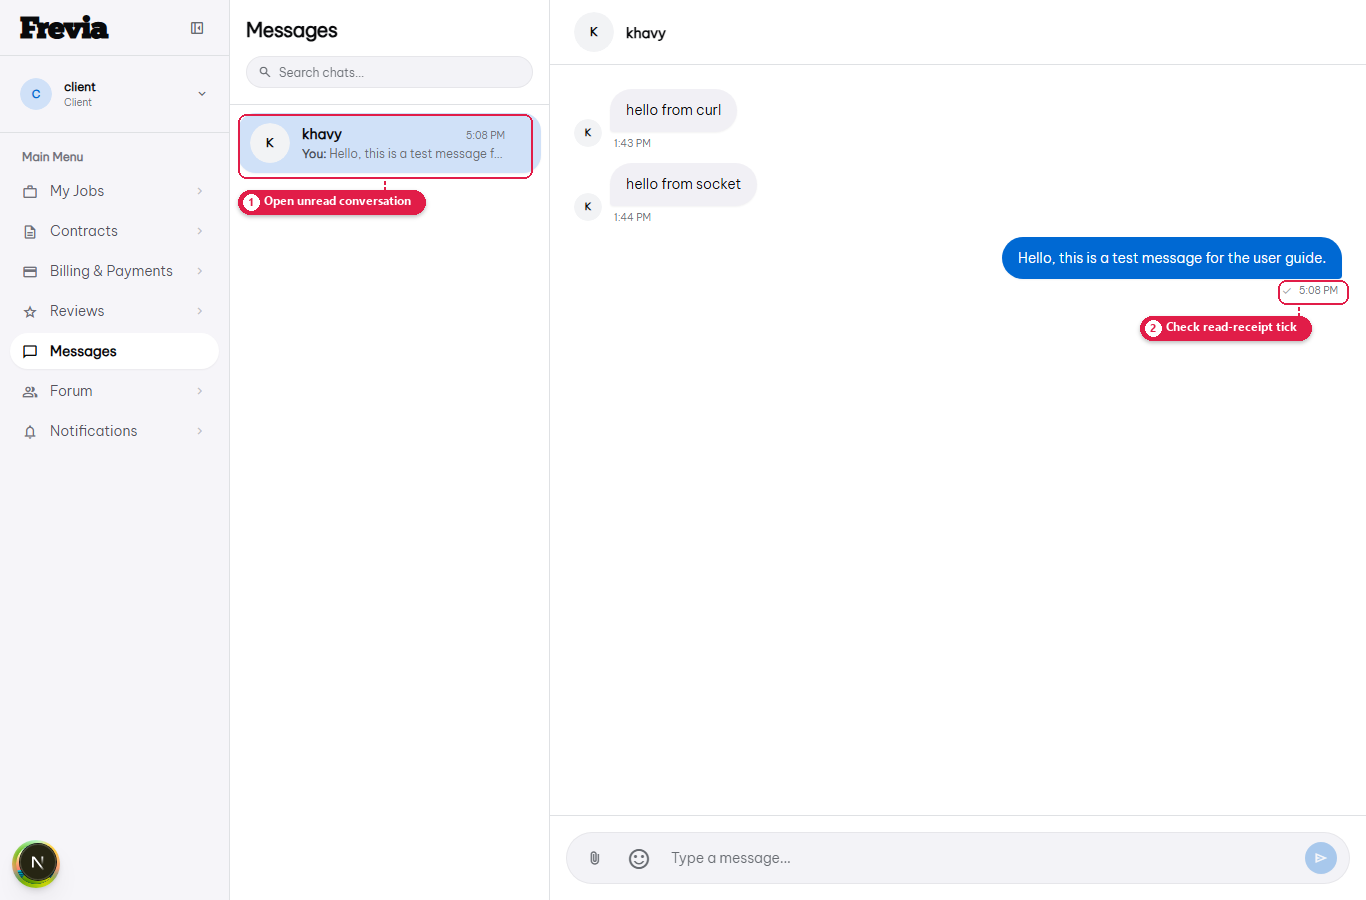
\includegraphics[width=0.90\textwidth]{images/conversation/c27_05_guide.png}
  \caption{Marking incoming messages as read}
\end{figure}
\Needspace{6\baselineskip}\paragraph{Step-by-Step User Guide:}
\begin{enumerate}[leftmargin=1.8em,itemsep=3pt]
  \item \rbadge{1} \textbf{Open Unread Thread:} Click a conversation showing a blue unread counter badge.
  \item \rbadge{2} \textbf{Verify Read Receipt:} Confirm the unread badge clears and read-receipt checkmarks update.
\end{enumerate}
\Needspace{6\baselineskip}\paragraph{After You Submit (Result \& Troubleshooting):}
\begin{itemize}[leftmargin=1.5em,itemsep=2pt]
  \item \textbf{What Happens Next:} Messages are marked \texttt{is\_read = true} and unread counts sync across sessions.
  \item \textbf{Troubleshooting \& Common Messages:} Network interruptions may delay read-receipt updates until reconnected.
\end{itemize}

\subsubsection{M27.06 -- Delete / Recall Message (UC-29.06)}
\begin{itemize}[leftmargin=1.5em,itemsep=2pt]
  \item \textbf{Screen Name \& Route Path:} Message Actions -- \texttt{/messages}.
  \item \textbf{Who Can Use This:} Client, Freelancer (Sender only).
  \item \Needspace{6\baselineskip}\textbf{Before You Begin:} User is the sender of the target message.
\end{itemize}
\begin{figure}[H]\centering
  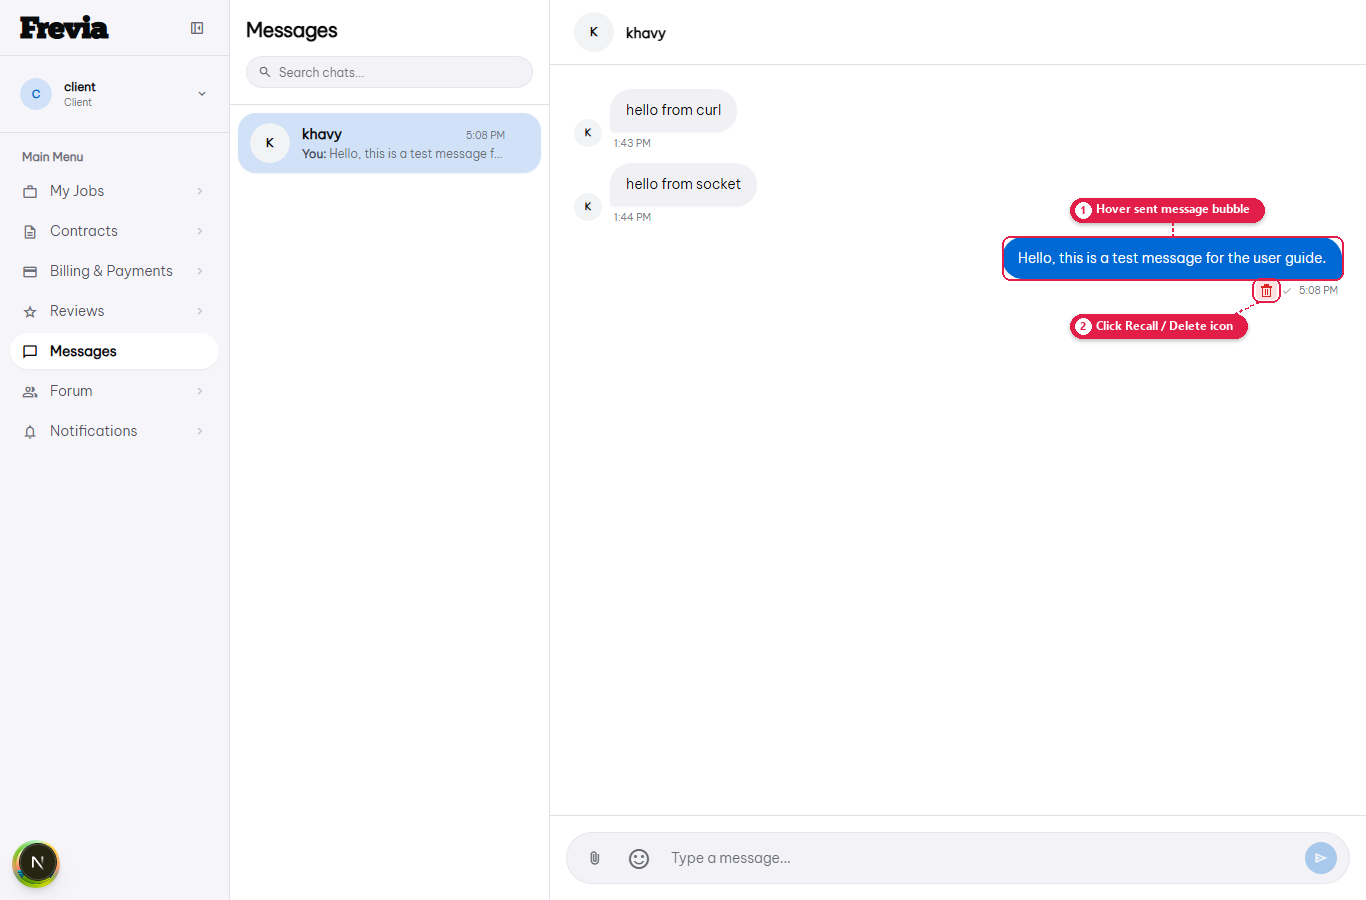
\includegraphics[width=0.90\textwidth]{images/conversation/c27_06_guide.png}
  \caption{Recalling a sent message}
\end{figure}
\Needspace{6\baselineskip}\paragraph{Step-by-Step User Guide:}
\begin{enumerate}[leftmargin=1.8em,itemsep=3pt]
  \item \rbadge{1} \textbf{Hover Sent Message:} Move your cursor over your sent blue message bubble to reveal the message action controls.
  \item \rbadge{2} \textbf{Click Recall / Delete Icon:} Click the red \textbf{Trash (Delete)} icon beside the timestamp to recall the message for both participants.
\end{enumerate}
\Needspace{6\baselineskip}\paragraph{After You Submit (Result \& Troubleshooting):}
\begin{itemize}[leftmargin=1.5em,itemsep=2pt]
  \item \textbf{What Happens Next:} The message is soft-deleted and hidden from the conversation UI.
  \item \textbf{Troubleshooting \& Common Messages:} Users cannot recall messages sent by the other participant.
\end{itemize}

\subsubsection{M27.07 -- Pin / Unpin Conversation (UC-29.07)}
\begin{itemize}[leftmargin=1.5em,itemsep=2pt]
  \item \textbf{Screen Name \& Route Path:} Conversation Options -- \texttt{/messages}.
  \item \textbf{Who Can Use This:} Client, Freelancer.
  \item \Needspace{6\baselineskip}\textbf{Before You Begin:} User has at least one active conversation.
\end{itemize}
\begin{figure}[H]\centering
  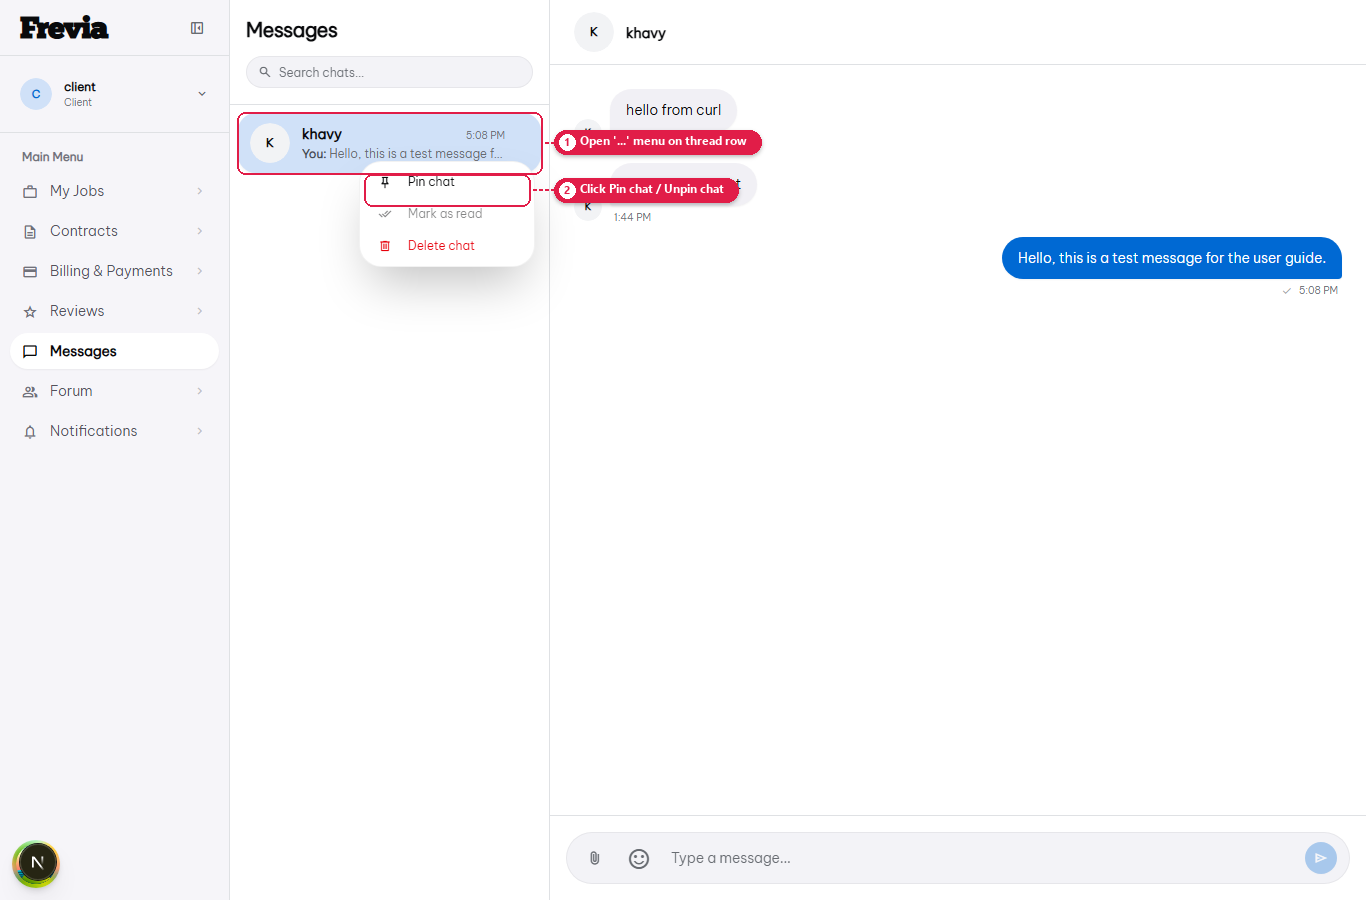
\includegraphics[width=0.90\textwidth]{images/conversation/c27_07_guide.png}
  \caption{Pinning or unpinning a conversation to top}
\end{figure}
\Needspace{6\baselineskip}\paragraph{Step-by-Step User Guide:}
\begin{enumerate}[leftmargin=1.8em,itemsep=3pt]
  \item \rbadge{1} \textbf{Open Thread Menu:} Click the \textbf{...} options menu on a conversation item in the sidebar.
  \item \rbadge{2} \textbf{Toggle Pin State:} Click \textbf{Pin Conversation} (or \textbf{Unpin}) to prioritize important chats.
\end{enumerate}
\Needspace{6\baselineskip}\paragraph{After You Submit (Result \& Troubleshooting):}
\begin{itemize}[leftmargin=1.5em,itemsep=2pt]
  \item \textbf{What Happens Next:} Pinned conversations stay anchored at the top of your inbox.
  \item \textbf{Troubleshooting \& Common Messages:} If the thread was deleted, pinning fails with a not-found alert.
\end{itemize}

\subsubsection{M27.08 -- Send File Attachment (UC-29.08)}
\begin{itemize}[leftmargin=1.5em,itemsep=2pt]
  \item \textbf{Screen Name \& Route Path:} Chat File Upload -- \texttt{/messages}.
  \item \textbf{Who Can Use This:} Client, Freelancer.
  \item \Needspace{6\baselineskip}\textbf{Before You Begin:} A conversation thread is active.
\end{itemize}
\begin{figure}[H]\centering
  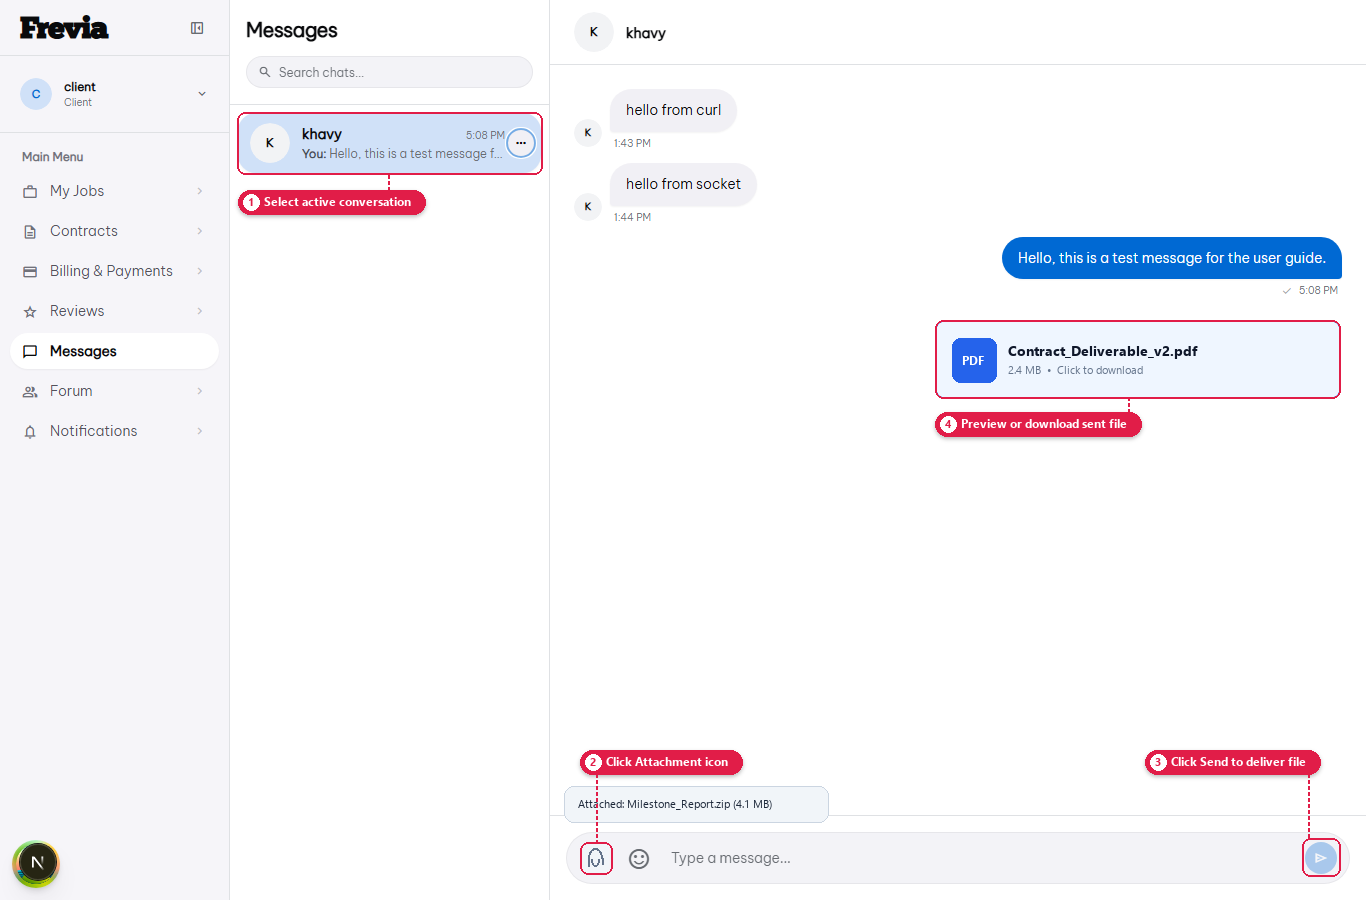
\includegraphics[width=0.90\textwidth]{images/conversation/c27_08_send_file_guide.png}
  \caption{Real-time Messaging and File Attachment Sharing (/messages)}
\end{figure}
\Needspace{6\baselineskip}\paragraph{Step-by-Step User Guide:}
\begin{enumerate}[leftmargin=1.8em,itemsep=3pt]
  \item \rbadge{1} \textbf{Select Conversation:} Choose the recipient thread from the left conversation sidebar.
  \item \rbadge{2} \textbf{Attach File:} Click the \textbf{Attachment (Paperclip)} icon to upload an image, PDF, DOCX, or archive (up to 25\,MB).
  \item \rbadge{3} \textbf{Send Attachment:} Click the blue \textbf{Send} button to transmit the file.
  \item \rbadge{4} \textbf{Preview or Download:} Click the rendered attachment card in chat to preview or download the file.
\end{enumerate}
\Needspace{6\baselineskip}\paragraph{After You Submit (Result \& Troubleshooting):}
\begin{itemize}[leftmargin=1.5em,itemsep=2pt]
  \item \textbf{What Happens Next:} The file is uploaded securely and rendered as a downloadable card for both participants.
  \item \textbf{Troubleshooting \& Common Messages:} Files exceeding 25\,MB or unsupported formats are blocked with a validation toast.
\end{itemize}

